\documentclass[journal,11pt]{IEEEtran}
\usepackage[T1]{fontenc}
\usepackage[utf8]{inputenc}
\usepackage{lmodern}
\usepackage[polish]{babel}
\usepackage{makeidx}
\usepackage{amsfonts}
\usepackage{graphicx}
\usepackage{url}
\usepackage{hyperref}

\title{Dodatkowe aplikacje w aparatach słuchowych: wystrzałowe gadżety czy przydatne ułatwienia}
\author{Bartłomiej~Bułat, Tomasz~Drzewiecki}

\begin{document}

%\markboth{Sztuczne Sieci Neuronowe, semestr letni 2011/2012, prowadzący: mgr
%inż. Tomasz Orzechowski}{}

\maketitle


\begin{abstract}
W~tym artykule opisano historyczne oraz współczesne aparaty słuchowe. Główny
nacisk położono na coraz częściej pojawiające się różne, dodatkowe funkcje
w~tych urządzeniach. Przedstawiono krótką historię aparatów słuchowych, od
skromnych początków do najnowszych generacji, które dzięki technologii
bezprzewodowej pozwalają na komunikację z~innymi urządzeniami elektrycznymi
takimi jak radio czy telefon komórkowy.
\end{abstract}

\begin{IEEEkeywords}
Aparaty słuchowe, innowacje, gadżet
\end{IEEEkeywords}

\section{Wstęp}

Ubytek słuchu to dla każdego człowieka utrudnienie życiowe. Zmysł słuchu
nieodzowny podczas komunikacji z~innymi ludźmi, a~także w poznawaniu
otaczającego nas świata. Człowiek również stworzył muzykę, której jedynym
zadaniem jest sprawienie człowiekowi przyjemności, której znaczny ubytek słuchu
pozbawia.

Z~wyżej wymienionych powodów ludzie starali się poprawiać słuch, dlatego już od
XVII wieku tworzono pierwsze urządzenia mające na celu pomoc osobom z~wadą słuchu.

Dopiero rozwój elektroniki pozwoli na konstruowanie bardziej zaawansowanych
rozwiązań, dlatego pierwsze elektryczne aparaty słuchowe powstały dopiero w XX
wieku.

Przez lata doskonalono te urządzenia i obecna technologia pozwala na bardzo
dużo. Aktualnie poza doskonaleniem działania układów mających na celu
przekazywać dźwięki z~otoczenia do ucha, rozwija się technologie wspomagające
działania aparatów, na których to, skupia się ten artykuł.

\section{Krótka historia aparatów słuchowych}

Pierwszymi urządzeniami skonstruowanymi w~celu poprawy jakości słyszenia były trąbki (rys. \ref{fig:trumpet}), których węższy koniec przykładano do ucha.

\begin{figure}
    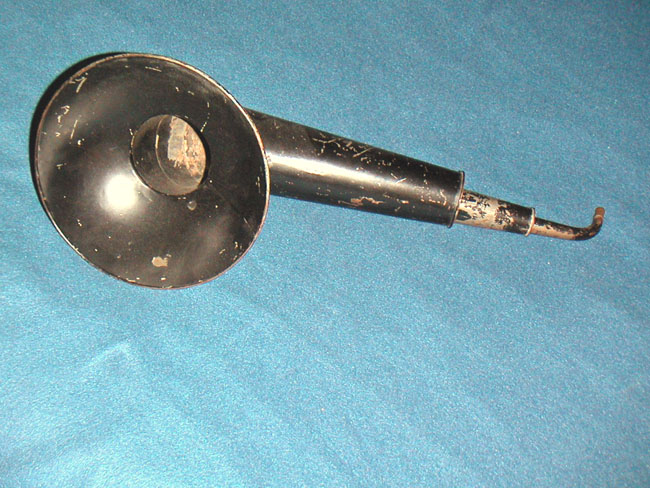
\includegraphics[width=0.5\textwidth]{trumpet}
    \caption{Trąbka słuchowa}
    \label{fig:trumpet}
\end{figure}

Pierwsze prace nad zastosowaniem sygnałów elektrycznych w~celu kompensacji wad
słuchu realizował Graham Bell. Pomimo tego, że nie udało mu się osiągnąć celu,
prowadzone przez niego badania znacząco pomogły mu wynalezienia telefonu.

W XX wieku skonstruowano pierwsze wzmacniacze elektryczne, których można było
użyć do konstrukcji elektrycznych urządzeń - już aparatów słuchowych. Pierwsze
maszyny były dużych rozmiarów zarówno ze względu na samo gabaryty elementów
elektronicznych, jak i~z~uwagi na baterię (rys. \ref{fig:siemens-old}).
Postępująca miniaturyzacja pozwoliła na stworzenie urządzeń kieszonkowych
dopiero w~latach czterdziestych XX wieku (rys. \ref{fig:electroear}). Wtedy to
powstawały kolejne generacje aparatów słuchowych, które coraz bardziej
upodabniały się do tych, znanych nam obecnie. W~latach sześćdziesiątych
stworzono pierwszy aparat zauszny, który obecnie jest najczęściej spotykanym
modelem.

\begin{figure}
    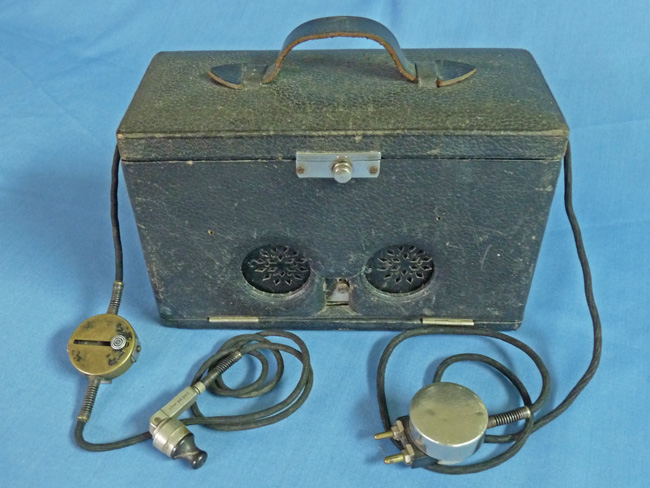
\includegraphics[width=0.5\textwidth]{siemens_old}
    \caption{Siemens/Fortiphone Model M-22 "Booster Flat" Carbon Hearing Aid}
    \label{fig:siemens-old}
\end{figure}

\begin{figure}
    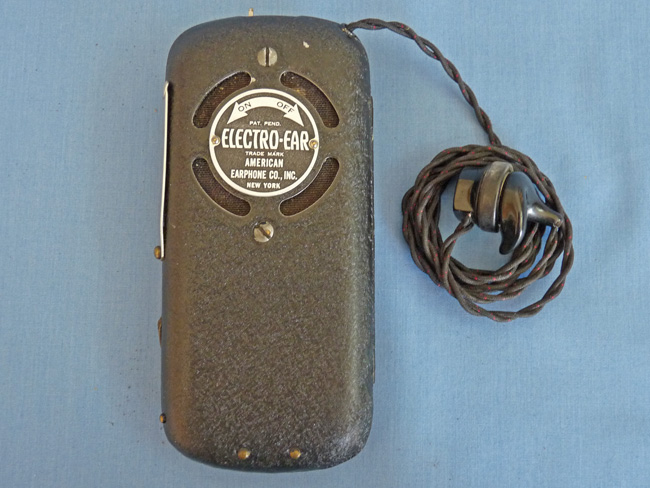
\includegraphics[width=0.5\textwidth]{electroear}
    \caption{Electro-Ear Model 5 Carbon Hearing Aid}
    \label{fig:electroear}
\end{figure}

Późniejsze aparaty stawały się coraz mniejsze i równocześnie charakteryzowały
się wyższą jakością wzmacnianego dźwięku. Tworzono lepsze procesory sygnałów,
z~lepszymi algorytmami przetwarzania oraz coraz popularniejszymi dodatkowymi aplikacjami.

\section{Współczesne aparaty słuchowe}

Obecnie funkcja poprawy jakości słyszenia staje się jedną z pośród wielu
dostępnych w aparatach słuchowych. Choć to ich główne zadanie, producenci
urządzeń starają się zachęcić pacjentów dodatkowymi aplikacjami, które
poprawiają działanie urządzenia (np. usuwanie sprzężeń zwrotnych), mają na celu
poprawę komfortu użytkowania (np. tłumienie szumu) lub poprawiają wrażenia
akustyczne (np. interpolacja dźwięku przestrzennego).

Poniżej są przedstawiono najczęściej spotykane rozszerzenia aparatów słuchowych.

\subsection{Tłumienie szumu}

Prawie wszystkie modele renomowanych firm dostępne na rynku oferują tłumienie
szumu i~redukcję hałasu. Ta funkcja jest dość pożądana w aparacie słuchowym
z~uwagi na możliwy długi i~trudny proces dopasowywania aparatu do pacjenta
oraz czas uczenia się pacjenta użytkowania urządzenia. Dotyczy to zwłaszcza
pacjentów, którzy wcześniej mieli znaczny ubytek słuchy lub byli całkowicie
głusi. Odbiór dźwięków z~użyciem aparatu znacznie odbiega od tego, do czego
pacjent był przyzwyczajony wcześniej. Dlatego korzystne jest ograniczenie
ilości i głośności dochodzących dźwięku, więc taka funkcja jest bardzo
przydatna.

Dodatkową funkcją jest redukcja szumu spowodowanego przez wiatr. Nie jest
jednak ona oferowana w~tak szerokiej gamie modeli, jak podstawowa redukcja
szumu. Nie jest to do końca uzasadnione, ponieważ szum wiatru wiejącego
w~mikrofon jest uciążliwy i bardzo utrudnia słyszenie. Być może jest to tylko
element marketingowy i~podstawowa funkcja tłumienia szumu pozwoli na rozumienie
mowy przy szumie wiatru. Tym niemniej ta funkcjonalność jest przydatna
i~powinna być obecna w~zdecydowanej większości aparatów.

\subsection{Usuwanie sprzężeń zwrotnych}

Podobnie jak moduł redukcji szumów, również ta funkcja jest obecna w~większości
modeli. Jest ona także istotna z punktu widzenia pacjenta. Podczas użytkowania
aparatu słuchowego mogą powstawać sprzężenia zwrotne, które są bardzo
nieprzyjemne. Dla niektórych pacjentów, zwłaszcza przy długim procesie
dopasowania do aparatu może być to odstraszające od używania urządzenia, mimo
wszystkich jego zalet. Dlatego należy ocenić tą funkcję jako pożądaną.

\subsection{Tryb działania zależny od otoczenia}

W niewielkiej liczbie aparatów można spotkać funkcję która zmienia sposób
działania urządzenia w~zależności od otoczenia. Pozwala to na dokładne
słyszenie w~różnych warunkach środowiska. Jest to próba odwzorowania sposobu
działania naturalnego ludzkiego słuchu, które pozwala człowieku na dokładne
rozumienie mowy w wielu sytuacjach (np. mimo hałasu w tramwaju możemy swobodnie
prowadzić rozmowę ze znajomym). W~związku z~tym tą funkcję także można uznać za
przydatną. Fakt, że jest ona obecna w mniejszej ilości aparatów pokazuje, że
bez niej można swobodnie słyszeć i~nie jest ona szczególnie pożądana.

\begin{figure}
    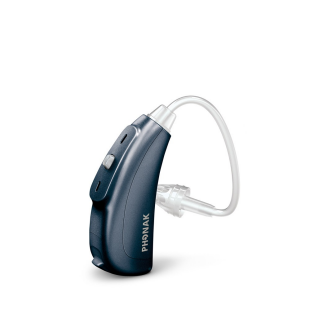
\includegraphics[width=0.5\textwidth]{phonak}
    \caption{Phonak Bolero Q}
    \label{fig:phonak}
\end{figure}

\subsection{Bezprzewodowa łączność}

Duża część aparatów pozwala na bezprzewodowe podłączenie się z~innym urządzeniem, mającym
możliwość nadawania dźwięku (radio, komputer osobisty). Pozwala to na
bezpośrednie przesłanie dźwięku ze źródła wprost do aparatu, dzięki czemu można
pominąć, powodujący istotne zakłócenia, ośrodek rozchodzenia się dźwięku -
powietrze. W takiej sytuacji aparat słuchowy działa jak słuchawki. Poprawia to
jakość dźwięku dochodzącego do pacjenta, który jest wtedy odbierany bez szumów
otoczenia. W~takiej sytuacji można również wyciszyć odgłosy odbierane z
zewnątrz, choć powstaje wtedy kwestia braku kontaktu z~otoczeniem. Dla komfortu
pacjenta może to mieć duże znaczenie, ponieważ dźwięk przesłany bezprzewodowo
bezpośrednio do urządzenia będzie lepszej jakości niż odbierany z mikrofonu
aparatu słuchowego.

Ta funkcja nie jest niezbędną do użytkowania aparatu, ponieważ dźwięk można
zawsze przesłać w sposób tradycyjny, ale wysoce podnosi komfort użytkowania
urządzenia.

\subsection{Fizyczna ochrona aparatu}

Wiele aparatów oferuję ochronę przed kurzem, wodą i~innymi zanieczyszczeniami.
Część posiada także powłokę antybakteryjną. Jest to przydatna funkcja, ponieważ
pozwala na korzystanie z aparatu w~deszczu lub podczas ćwiczeń (np. biegania).
Nawet podczas normalnego użytkowania zdarzają się wypadki, kiedy aparat może
zostać zabrudzony lub zalany. Ułatwia to pacjentom prowadzenie normalnego trybu
życia, pozwalając na korzystanie z urządzenia w każdych warunkach. Ma to
również wpływ na bezpieczeństwo użytkownika aparatu, pozwalając słyszeć
niezależnie od aury i środowiska.

\subsection{Dodatkowe akcesoria}

Niektórzy producenci do urządzenia oferują możliwość użycia dodatkowych
akcesoriów. Są to między innymi: piloty, służące do sterowania aparatem,
adaptery do różnych urządzeń pozwalające na bezprzewodową łączność, dodatkowe
lub oferujące większą pojemność baterie, specjalne ładowarki do baterii lub też
łączniki do okularów. Oferowane akcesoria nieco różnią się pomiędzy
poszczególnymi firmami, ale w~działaniu są bardzo podobne. Niektóre z
akcesoriów są konieczne, by skorzystać z~pełnych możliwości aparatu.


\begin{figure}
    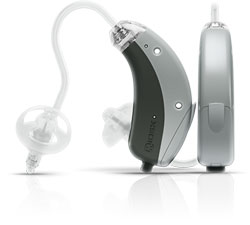
\includegraphics[width=0.5\textwidth]{widex}
    \caption{Widex SUPER}
    \label{fig:widex}
\end{figure}

\subsection{Obsługa dwóch aparatów}

W~przypadku posiadania dwóch aparatów, bardziej zaawansowane modele oferują
dźwięk przestrzenny. Zapewnia to wrażenia podobne do tych naturalnie
występujących u ludzi słyszących: kierunek, skąd, dobiega dźwięk, orientacja
przestrzenna; zapewnia również lepszą orientację przestrzenną. Taka funkcja
jest szczególnie przydatna dla osób, które mają wadę w~obydwu uszach, lecz jest
zupełnie nieistotna dla osób z~ubytkiem w~tylko jednym uchu.

\subsection{Obsługa telefonu w przypadku dwóch aparatów}

Modele droższe oferują również, w~przypadku posiadania dwóch aparatów,
odpowiednie zachowanie, gdy wykryją rozmowę telefoniczną (dźwięk dobiegający
tylko do jednego ucha). W~tej sytuacji urządzenia zachowują się różnie. Modele
firmy Phonak przekazują dźwięk do drugiego ucha, więc pacjent odbiera rozmowę,
tak jakby rozmówca był tuż obok. Aparaty firmy Bernafon wyciszają urządzenie
przy drugim uchu, więc szum otoczenia staje się niesłyszalny. Podobnie jak
w~przypadku dodatku powyżej ta funkcja jest dostępna dla osób posiadających dwa
aparaty słuchowe, lecz niewątpliwie jest przydatna przy korzystaniu z
telefonu.

\subsection{Wygląd}

Większość producentów pozwala na personalizację wyglądu urządzenia. Zwykle
dostępnych jest od kilku do kilkunastu kolorów do wyboru. Może to być istotne
dla komfortu pacjenta i~akceptacji konieczności użycia aparatu. Obecnie
urządzenia są małe, bardzo łatwe do ukrycia, co również może zmniejszyć
dyskomfort psychiczny pacjenta.

\subsection{Specjalne funkcje}

Aparat firmy Bernafon oferuje specjalne tryby: do słuchania muzyki na żywo oraz
do oglądania filmów w~kinie. Takie tryby mają na celu poprawienie wrażeń
słuchowych. W~żaden sposób nie są konieczne do poprawnego działania aparatu. 

\section{Podsumowanie}

Aparaty słuchowe, odkąd stały się małymi komputerami, wzbogacane są o różne
dodatkowe funkcjonalności, zwykle mające na celu poprawę komfortu użytkowania.
Istnieje też szereg funkcji, które nie mają nic wspólnego z ideą przywrócenia
zdolności słyszenia niedosłyszącym. Choć wiele wymienionych tu rozszerzeń można
nazwać przydatnymi ułatwieniami dla pacjenta, część z nich to tylko wystrzałowe
gadżety, dodatkowo ułatwiające życie ludziom z wadami słuchu.

\begin{thebibliography}{123}
    \bibitem{Interton}, Strona firmy Interton.
        \url{http://www.interton-polska.pl/}
    \bibitem{Oticon}, Strona firmy Oticon
        \url{http://www.oticon.pl/}
    \bibitem{Widex}, Strona firmy Widex
        \url{http://www.widex.pl/pl-pl/}
    \bibitem{Phonak}, Strona firmy Phonak
        \url{http://www.phonakpro.com/pl/}
    \bibitem{Bernafon}, Strona firmy Bernafon
        \url{http://www.bernafon.pl/Consumers.aspx}
    \bibitem{Siemens}, Strona firmy Siemens
        \url{http://hearing.siemens.com/Global/en/products/hearing-products.html}
    \bibitem{AudioService}, Strona firmy Audio Service
        \url{http://www.audioservice.pl/}
    \bibitem{Beltone}, Strona firmy Beltone
        \url{http://www.beltone.com/index.aspx}
    \bibitem{hearingaidmuseum}, Muzeum aparatów słuchowych
        \url{http://www.hearingaidmuseum.com/gallery.htm}
\end{thebibliography}

\end{document}
